

\section*{Глава 1. Анализ предметной области}
\addcontentsline{toc}{section}{Глава 1. Анализ предметной области}
\stepcounter{section}

\subsection{Обзор существующих аниме-платформ (аналоги, функциональность)}

На современном рынке онлайн-энциклопедий и сообществ, посвящённых аниме, можно выделить несколько ключевых проектов: узкоспециализированные базы данных (AniDB, Anilist) и полнофункциональные социальные платформы (Shikimori, MyAnimeList). Проведём сравнение наиболее популярных решений в таблице~\ref{tab:anime_platforms}.

\begin{table}[ht!]
	\small
	\centering
	\caption{Сравнительный анализ аниме-платформ}
	\label{tab:anime_platforms}
	\begin{tabular}{|l|c|c|c|}
		\hline
		\textbf{Название} & \textbf{Тип рекомендаций} & \textbf{Архитектура} & \textbf{API} \\ \hline
		Shikimori & Только оценки & Монолит & REST, GraphQL \\ \hline
		MyAnimeList & Только оценки & Монолит & Ограничен \\ \hline
		AniDB & Нет & Монолит & Есть \\ \hline
		Anilist & Базовая коллаборативная & Монолит (SPA) & GraphQL \\ \hline
	\end{tabular}
\end{table}

Проведенный анализ (см. табл.~\ref{tab:anime_platforms}) показывает, что существующие платформы, включая такие крупные, как Shikimori и Anilist, имеют монолитную архитектуру. Системы рекомендаций реализованы примитивно: либо на основе средних оценок, либо отсутствуют вовсе. Отсутствие гибридного подхода и микросервисного разделения подтверждает актуальность разработки предлагаемой платформы с изолированным сервисом рекомендаций.
\\
\subsection{Анализ целевой аудитории}

Для обоснования требований к интерфейсу и функционалу проведён анализ целевой аудитории. По данным открытых исследований (Anime News Network, Statista), ядро аудитории аниме-платформ — люди в возрасте 18–30 лет, с равномерным распределением по полу. На рисунке~\ref{fig:age_gender} представлена возрастная и гендерная структура.

\begin{figure}[ht!]
	\centering
	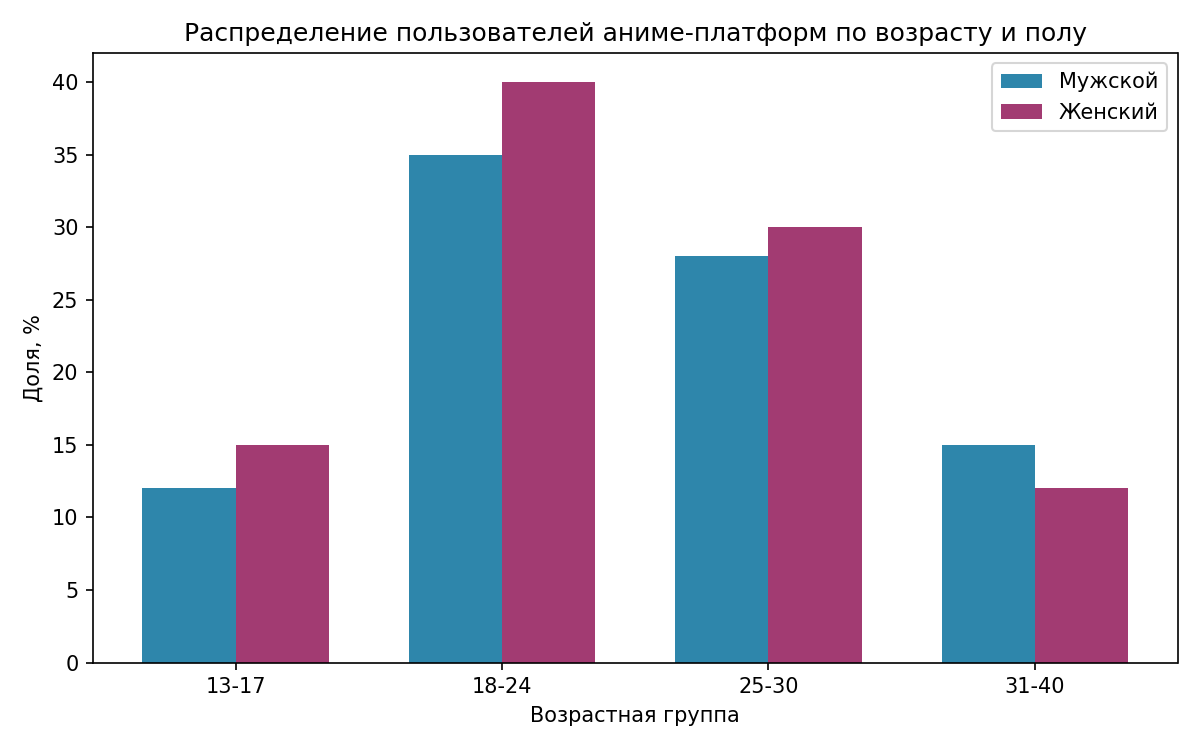
\includegraphics[width=0.7\textwidth]{age_gender_chart.png}
	\caption{Распределение пользователей по возрасту и полу}
	\label{fig:age_gender}
\end{figure}

Далее, для сегментации по жанровым предпочтениям (рисунок~\ref{fig:genre_heatmap}) мы выделили три типа аудитории:
\begin{itemize}
	\item \textbf{Новички} — предпочитают приключения, комедии, повседневность.
	\item \textbf{Опытные зрители} — экшен, драма, психология.
	\item \textbf{Энтузиасты} — сэйнэн, дзёсэй, экспериментальное.
\end{itemize}

\begin{figure}[ht!]
	\centering
	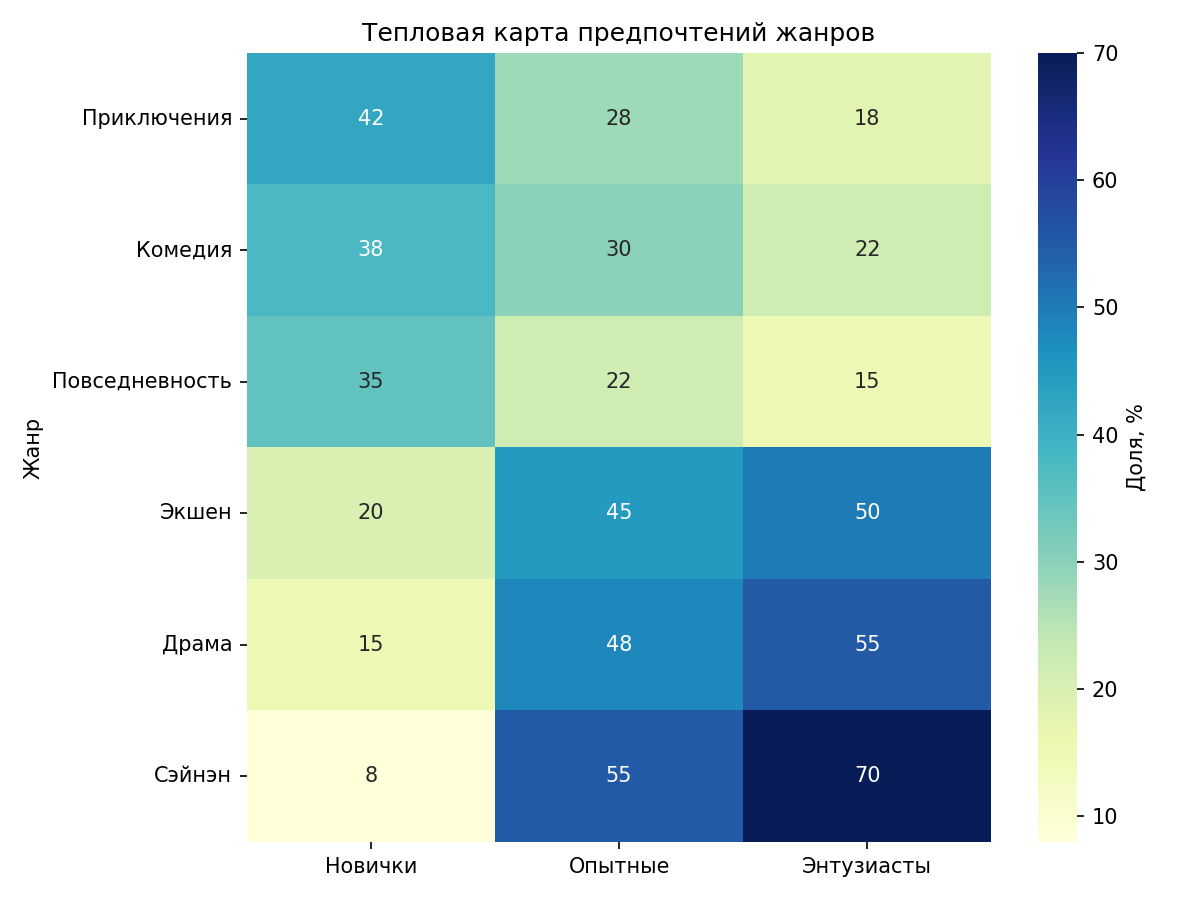
\includegraphics[width=0.8\textwidth]{genre_heatmap.png}
	\caption{Предпочтение жанров по группам аудитории}
	\label{fig:genre_heatmap}
\end{figure}
\\
\subsection{Анализ программных инструментов разработки}

Архитектура проекта предполагает четыре микросервиса: фронтенд-сервис (FastAPI), контент-сервис (Python), сервис аутентификации и пользователей (Go) и движок рекомендаций (Python).

\textbf{Выбор языка и стека для сервиса аутентификации и пользователей}

Выбор Go обусловлен:
\begin{itemize}
	\item Высокой производительностью при работе с JWT и сессиями (сотни тысяч concurrent-соединений);
	\item Простой сборкой в статический бинарный файл — удобно для контейнеризации;
	\item Надёжной стандартной библиотекой для HTTP и криптографии.
\end{itemize}

\textbf{Выбор инструментов для контент-сервиса и сервиса рекомендаций}

Python выбран благодаря богатой экосистеме для работы с данными:
\begin{itemize}
	\item \textbf{FastAPI} — асинхронный фреймворк с автоматической генерацией OpenAPI;
	\item \textbf{SQLAlchemy} — ORM для работы с PostgreSQL;
	\item \textbf{pandas / numpy / scikit-learn} — для реализации коллаборативной и контентной фильтрации.
\end{itemize}

\textbf{Выбор инструментов для Frontend Service}

Frontend Service реализован на \textbf{FastAPI + Jinja2} + статические HTML/CSS/JS. Это позволит отдавать полностью готовые страницы, уменьшая нагрузку на клиента.

Таким образом, выбранный стек удовлетворяет требованиям к масштабируемости, скорости разработки и лёгкости развёртывания.
\\
\subsection{Формулировка цели и задач работы}

На основе проведённого анализа (подразделы 1.1-1.3) и выявленных недостатков существующих решений (отсутствие гибридных рекомендаций, монолитность) сформулирована цель исследования.

\textbf{Цель работы} — разработать веб-приложение (аниме-энциклопедию), обеспечивающее просмотр информации о произведениях, ведение пользовательского избранного, комментирование и получение персонализированных рекомендаций на основе гибридного подхода.

Для достижения поставленной цели необходимо решить следующие \textbf{задачи}:
\begin{enumerate}
	\item Провести сравнительный анализ существующих аниме-платформ и алгоритмов рекомендаций.
	\item Разработать архитектуру клиент-серверного приложения на основе микросервисов и спроектировать базу данных для хранения информации об аниме, пользователях, комментариях и избранном.
	\item Реализовать программные модули для управления пользователями, аутентификации (JWT), CRUD-операций с аниме и новостями.
	\item Разработать сервис рекомендаций, сочетающий content-based и коллаборативную фильтрацию, и интегрировать его с основным приложением.
	\item Внедрить каркас фронтенда для отображения страниц каталога, карточек аниме, системы комментариев и личного кабинета.
	\item Настроить контейнеризацию (Docker) и оркестрацию (Docker Compose) для всех четырёх сервисов и Nginx.
	\item Провести тестирование разработанной системы в условиях, приближенных к реальным.
\end{enumerate}